\documentclass{../template/tp}
\usepackage[utf8x]{inputenc}

\usepackage[english]{babel}
\usepackage[T1]{fontenc}

\usepackage{graphicx}
\usepackage{amssymb}
\usepackage{amsmath}
\usepackage{wasysym} %smiley
\usepackage{hyperref}% hyperliens
\usepackage{tikz}
\usetikzlibrary{babel,positioning,calc}
\usepackage[]{circuitikz}
\usepackage{textcomp}
% \usepackage{minted}
\usepackage[long]{datetime}
\usepackage{gensymb} % \ohm, celsius
\usepackage{framed}
\usepackage{pdfpages}
\usepackage{todonotes}
\usepackage{enumitem}
\usepackage{ marvosym }
\usepackage{qrcode}%Don't forget to escape the "#", as the href package requires.
\usepackage{tabularx}

\usepackage{mathastext} % math as standfard text : units are respecting typography conventions.
\usepackage{fancyhdr}
% \langexam{frenchb}

\usepackage{subcaption}

\graphicspath{{imgs/}}

\newcommand{\labTitle}{GRAFCET}
\newcommand{\labNumber}{3}

\newcommand{\version}{v2.0.0}

\newcommand{\mnemonic}{ELEC-H-516}
\newcommand{\courseName}{Programmable Logic Controllers}

\newboolean{koriG}
\ifx\koriG\undefined
\correction{false}
\else
\correction{true}
\fi

% \correction{false}
% \correction{true}

\author{The Fantastic Four}


%% fancy header & foot
\pagestyle{fancy}
\lhead{[\mnemonic] \courseName\\ LABO  \labNumber :  \labTitle}
\rhead{\version\\ page \thepage}
\cfoot{}
%%

\pdfinfo{
/Author (ULB -- BEAMS)
/Title (Labo \labNumber \mnemonic, \labTitle)
/ModDate (D:\pdfdate)

}
\hypersetup{
pdftitle={Labo \labNumber [\mnemonic] \courseName : \labTitle},
pdfauthor={©2017 ULB - BEAMS  },
pdfsubject={\labTitle}
}


\setlength{\parskip}{0.5cm plus4mm minus3mm} %espacement entre §
\setlength{\parindent}{0pt}

\begin{document}

\tptitle{}{Labo \labNumber : \labTitle}

\vspace{-1cm}

\rule{\linewidth}{.5pt}

\Question{
	The process is described as follows: product A is first weighted until the balance reaches the point a, and then is placed in the reservoir. The same procedure is repeated for product B. After the product B is placed in the reservoir, 2 solid blocks of the product D are placed in
	the reservoir. When all three products are in the reservoir the valve C has been opened to provide liquid to the reservoir. The amount of the liquid is controlled by the time the valve is opened (or until given level is reached). Once the liquid is in the mixer will steer everything for 30s. The reservoir is emptied and the system is ready to start a new sequence.
	
	Build the SFC that controls the process described above and provide the necessary simulation environment.
	
	\begin{figure}[h]
		\centering
		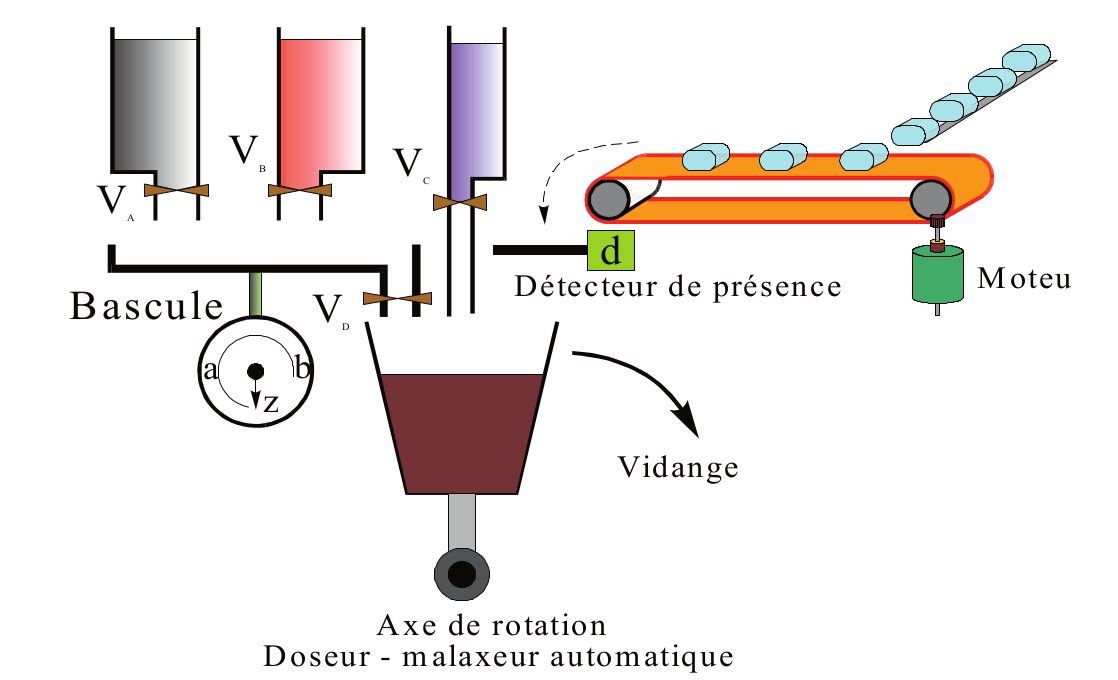
\includegraphics[width=0.8\linewidth]{exo1}
		\caption{}
		\label{grafcet}
	\end{figure}

}{}

\newpage

\Question{
	Imagine a system of wagons that need to transport some useful load from multiple points $ A_{i} $ to $ C $. 
	The disembarking position $ C $ is common for few wagons.
	At position $ A_{i} $, a worker manually charge the wagon, then presses the $ d_{Ai} $ button to indicate that he finished.
	The wagon is then moved toward a temporary position $ B_{i} $.
	Since only one wagon at a time can discharge its load, it should wait at $ B_{i} $ until $ C $ is freed.
	The discharge of the cart takes around 20 seconds.
	For this exercise consider the case of two wagons as illustrated bellow.

	Build the SFC that controls the process and provide the necessary simulation environment.
	
	\begin{figure}[h]
		\centering
		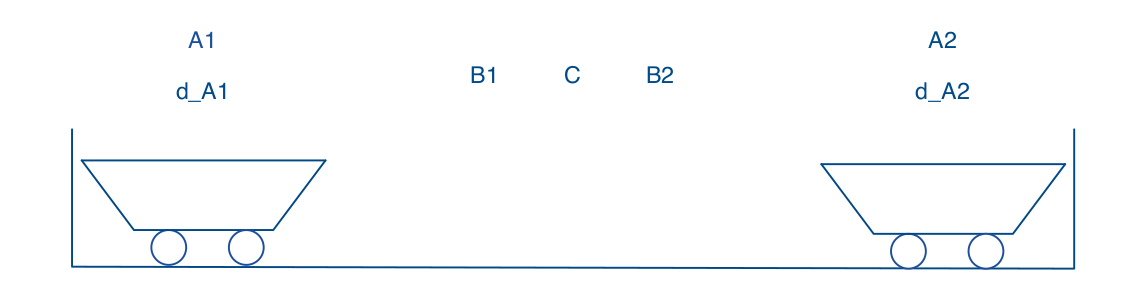
\includegraphics[width=0.8\linewidth]{exo2}
		\caption{}
		\label{grafcet}
	\end{figure}
}{}


\end{document}